\documentclass[tikz,border=10pt]{standalone}
\usepackage{mathrsfs}
\usetikzlibrary{decorations.pathmorphing}
    % this is for graphics. e.g. rectangle on title page
\usetikzlibrary{3d}
\usetikzlibrary{backgrounds}
\usetikzlibrary{arrows,shapes,positioning,shadows,trees,mindmap}
\usetikzlibrary{tikzmark}
\usetikzlibrary{calc,math}

\usepackage{tikz-3dplot}
\usepackage{pgfplots}
\pgfplotsset{compat = newest}
%\usepgfplotslibrary{colormaps}
\usepgflibrary{shapes.geometric}

\usepackage[edges]{forest}
\usetikzlibrary{arrows.meta}
\colorlet{linecol}{black!75}
\usepackage{xkcdcolors} % xkcd colors

\usetikzlibrary{patterns}
\tikzset{>={Stealth[inset=0pt,angle=20:10pt]}}


\tikzset{zigzag/.style={decorate,decoration=zigzag}}


\begin{document}
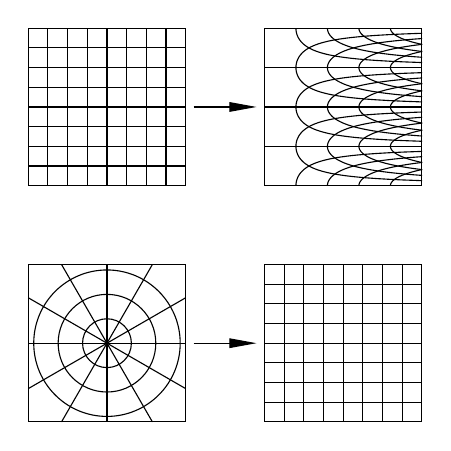
\begin{tikzpicture}
    \draw[->] (1.1,0)--(1.9,0);
    \draw[->] (1.1,-3)--(1.9,-3);
        \draw (-1,1) --(1,1)--(1,-1)--(-1,-1)--cycle;
        \draw (4,1) --(4,-1)--(2,-1)--(2,1)--cycle;
        \draw (4,-2) --(4,-4)--(2,-4)--(2,-2)--cycle;
    \foreach \N in {-0.75,-0.5,...,0.75}
    {\draw (\N,-1)--(\N,1);
    \draw (-1,\N)--(1,\N);
    \draw (\N+3,-4)--(\N+3,-2);
    \draw (2,\N-3)--(4,\N-3);
    }
    \foreach \O in {1,2,3}
    {\draw (0,-3) circle(0.31*\O);}
    \foreach \M in {0,30,...,360}
    {
    \draw[domain=0:{sec(\M-floor(\M/90+1/2)*90)},samples=2,variable=\x] plot({\x*cos(\M)},{\x*sin(\M)-3});
    }
    \draw (-1,-2) --(1,-2)--(1,-4)--(-1,-4)--cycle;
    \def\s{50}
    \foreach \F in {0,1,2,3}
    {
    \draw[domain=0:1.37,samples=\s,variable=\x] 
    plot({1/cos(\x*180/pi)/2.5+2},{(\x+\F*pi/2)/pi-1});
    \draw[domain=0:1.16,samples=\s,variable=\x] 
    plot({2/cos(\x*180/pi)/2.5+2},{(\x+\F*pi/2)/pi-1});
    \draw[domain=0:0.93,samples=\s,variable=\x] 
    plot({3/cos(\x*180/pi)/2.5+2},{(\x+\F*pi/2)/pi-1});
    \draw[domain=0:0.64,samples=\s,variable=\x] 
    plot({4/cos(\x*180/pi)/2.5+2},{(\x+\F*pi/2)/pi-1});
    }
    \foreach \F in {1,2,3,4}{
    \draw[domain=0:1.37,samples=\s,variable=\x] 
    plot({1/cos(\x*180/pi)/2.5+2},{(-\x+\F*pi/2)/pi-1});
    \draw[domain=0:1.16,samples=\s,variable=\x] 
    plot({2/cos(\x*180/pi)/2.5+2},{(-\x+\F*pi/2)/pi-1});
    \draw[domain=0:0.93,samples=\s,variable=\x] 
    plot({3/cos(\x*180/pi)/2.5+2},{(-\x+\F*pi/2)/pi-1});
    \draw[domain=0:0.64,samples=\s,variable=\x] 
    plot({4/cos(\x*180/pi)/2.5+2},{(-\x+\F*pi/2)/pi-1});
    }
    \foreach \F in {-1,0,1}
    {\draw (2,{\F/2})--(4,{\F/2});}
    \end{tikzpicture}
\end{document}